% ============================================================
% SF-CARS Dispersion Simulation — Beamer Presentation (v2)
% Audience: Master students in photonics
% Theme: Metropolis (16:9)
% Rule: slide title = take-away sentence; figures fill the slide
% ============================================================
\documentclass[aspectratio=169, 11pt]{beamer}

\usetheme[progressbar=frametitle, block=fill]{metropolis}

% ── Packages ────────────────────────────────────────────────
\usepackage{graphicx}
\usepackage{amsmath, amssymb}
\usepackage{booktabs}
\usepackage{siunitx}
\usepackage{xcolor}
\usepackage{tikz}
\usetikzlibrary{arrows.meta, positioning, shapes.geometric, fit, calc}
\usepackage{pgfplots}
\pgfplotsset{compat=1.18}

% ── Colours ─────────────────────────────────────────────────
\definecolor{mblue}{RGB}{0, 90, 160}
\definecolor{morange}{RGB}{220, 100, 0}
\definecolor{mgreen}{RGB}{30, 140, 60}
\definecolor{mgray}{RGB}{100, 100, 100}

% ── Macros ───────────────────────────────────────────────────
\newcommand{\wn}{\,\text{cm}^{-1}}
\newcommand{\Epump}{E_{\mathrm{pump}}}
\newcommand{\Estokes}{E_{\mathrm{Stokes}}}
\newcommand{\neff}{n_{\mathrm{eff}}}

% ── Title ────────────────────────────────────────────────────
\title{Chirping Laser Pulses for Spectral-Focusing CARS}
\subtitle{Dispersion, Resolution, and Signal Trade-offs}
\author{Justine Major}
\date{\today}
\institute{Maîtrise en biophotonique}

% ============================================================
\begin{document}
% ============================================================

% ──────────────────────────────────────────────────────────────
% 1. TITLE
% ──────────────────────────────────────────────────────────────
\maketitle

% ──────────────────────────────────────────────────────────────
% 2. CARS PHYSICS
% ──────────────────────────────────────────────────────────────
\begin{frame}{CARS detects lipid bond vibrations coherently, without labels}
  \begin{columns}[c]
    \column{0.50\textwidth}
      \centering
      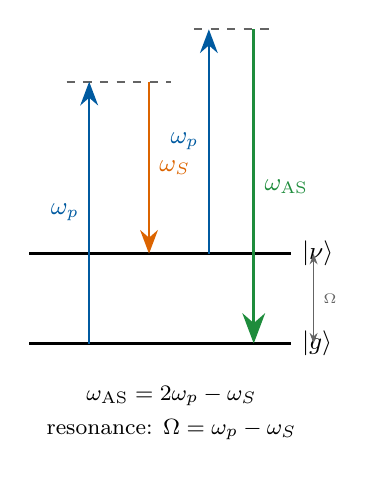
\begin{tikzpicture}[scale=0.95]
        % Ground state
        \draw[very thick] (0,0) -- (3.5,0)
          node[right, font=\small] {$|g\rangle$};
        % Raman level
        \draw[very thick] (0,1.2) -- (3.5,1.2)
          node[right, font=\small] {$|\nu\rangle$};
        % Virtual states
        \draw[thick, dashed, mgray] (0.5,3.5) -- (1.9,3.5);
        \draw[thick, dashed, mgray] (2.2,4.2) -- (3.2,4.2);
        % Pump up
        \draw[-{Stealth[scale=1.3]}, mblue, thick]
          (0.8,0) -- (0.8,3.5)
          node[midway, left, font=\small] {$\omega_p$};
        % Stokes down
        \draw[-{Stealth[scale=1.3]}, morange, thick]
          (1.6,3.5) -- (1.6,1.2)
          node[midway, right, font=\small] {$\omega_S$};
        % Probe up
        \draw[-{Stealth[scale=1.3]}, mblue, thick]
          (2.4,1.2) -- (2.4,4.2)
          node[midway, left, font=\small] {$\omega_p$};
        % Anti-Stokes down
        \draw[-{Stealth[scale=1.3]}, mgreen, very thick]
          (3.0,4.2) -- (3.0,0)
          node[midway, right, font=\small] {\textbf{$\omega_{\mathrm{AS}}$}};
        % Raman arrow
        \draw[{Stealth[scale=0.8]}-{Stealth[scale=0.8]}, mgray]
          (3.8,0) -- (3.8,1.2)
          node[midway, right, font=\tiny] {$\Omega$};
        % Resonance condition
        \node[font=\footnotesize, align=center] at (1.9,-0.7)
          {$\omega_{\mathrm{AS}} = 2\omega_p - \omega_S$};
        \node[font=\footnotesize, align=center] at (1.9,-1.15)
          {resonance: $\Omega = \omega_p - \omega_S$};
      \end{tikzpicture}

    \column{0.47\textwidth}
      \centering
      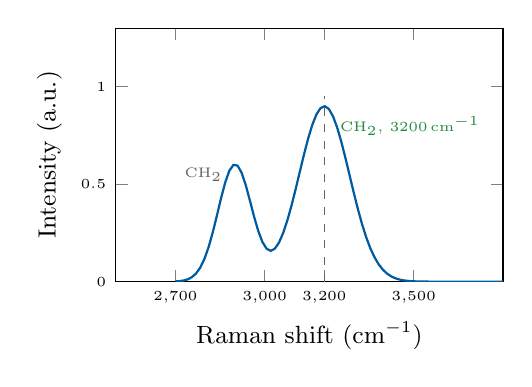
\begin{tikzpicture}
        \begin{axis}[
          width=6.5cm, height=4.8cm,
          xlabel={Raman shift (\(\text{cm}^{-1}\))},
          ylabel={Intensity (a.u.)},
          xmin=2500, xmax=3800,
          ymin=0, ymax=1.3,
          xtick={2700, 3000, 3200, 3500},
          xticklabel style={font=\tiny},
          yticklabel style={font=\tiny},
          xlabel style={font=\small},
          ylabel style={font=\small},
          axis line style={thin},
          tick style={thin},
        ]
          \addplot[thick, mblue, samples=80, domain=2700:3800]
            {0.9*exp(-((x-3200)/120)^2) + 0.6*exp(-((x-2900)/80)^2)};
          \draw[dashed, mgray] (axis cs:3200,0) -- (axis cs:3200,0.95);
          \node[font=\tiny, anchor=west, mgreen]
            at (axis cs:3220, 0.80) {CH$_2$, 3200\,cm$^{-1}$};
          \node[font=\tiny, anchor=east, mgray]
            at (axis cs:2890, 0.55) {CH$_2$};
        \end{axis}
      \end{tikzpicture}

      \vspace{0.3em}
      {\small Pump: \SI{803}{nm} \quad Stokes: \SI{1041}{nm}
             \quad AS: \SI{654}{nm}}
  \end{columns}
\end{frame}

% ──────────────────────────────────────────────────────────────
% 3. SPECTRAL FOCUSING CONCEPT
% ──────────────────────────────────────────────────────────────
\begin{frame}{Stretching both pulses with glass makes the instantaneous frequency difference constant}
  \centering
  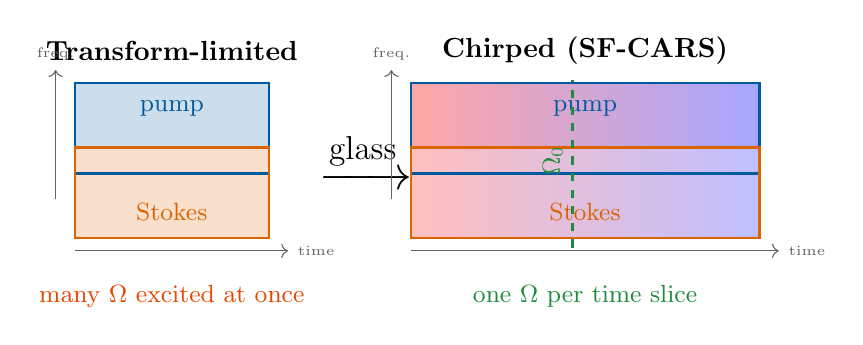
\begin{tikzpicture}[scale=0.82]
    % --- TL ---
    \node[font=\normalsize\bfseries] at (1.8, 5.1) {Transform-limited};
    \fill[mblue!20]   (0.3,3.2) rectangle (3.3,4.6);
    \fill[morange!20] (0.3,2.2) rectangle (3.3,3.6);
    \draw[mblue,   thick] (0.3,3.2) rectangle (3.3,4.6);
    \draw[morange, thick] (0.3,2.2) rectangle (3.3,3.6);
    \node[mblue,   font=\small] at (1.8,4.2) {pump};
    \node[morange, font=\small] at (1.8,2.6) {Stokes};
    \draw[->, mgray] (0.0,2.8) -- (0.0,4.8) node[above, font=\tiny] {freq.};
    \draw[->, mgray] (0.3,2.0) -- (3.6,2.0) node[right, font=\tiny] {time};
    \node[morange!70!red, font=\small] at (1.8,1.3) {many $\Omega$ excited at once};

    % --- arrow ---
    \node[font=\LARGE] at (4.8,3.4) {$\xrightarrow{\mathrm{glass}}$};

    % --- Chirped ---
    \node[font=\normalsize\bfseries] at (8.2,5.1) {Chirped (SF-CARS)};
    \shade[left color=red!35, right color=blue!35]
          (5.5,3.2) -- (10.9,3.2) -- (10.9,4.6) -- (5.5,4.6) -- cycle;
    \shade[left color=red!25, right color=blue!25]
          (5.5,2.2) -- (10.9,2.2) -- (10.9,3.6) -- (5.5,3.6) -- cycle;
    \draw[mblue,   thick] (5.5,3.2) rectangle (10.9,4.6);
    \draw[morange, thick] (5.5,2.2) rectangle (10.9,3.6);
    \node[mblue,   font=\small] at (8.2,4.2) {pump};
    \node[morange, font=\small] at (8.2,2.6) {Stokes};
    \draw[->, mgray] (5.2,2.8) -- (5.2,4.8) node[above, font=\tiny] {freq.};
    \draw[->, mgray] (5.5,2.0) -- (11.2,2.0) node[right, font=\tiny] {time};
    % one time slice
    \draw[mgreen, very thick, dashed] (8.0,2.05) -- (8.0,4.65);
    \node[mgreen, font=\small, rotate=90] at (7.7,3.4) {$\Omega_0$};
    \node[mgreen, font=\small] at (8.2,1.3) {one $\Omega$ per time slice};
  \end{tikzpicture}
\end{frame}

% ──────────────────────────────────────────────────────────────
% 4. TL PUMP — initial
% ──────────────────────────────────────────────────────────────
\begin{frame}{The pump starts transform-limited: all 80 spectral slices peak together at $t=0$}
  \centering
  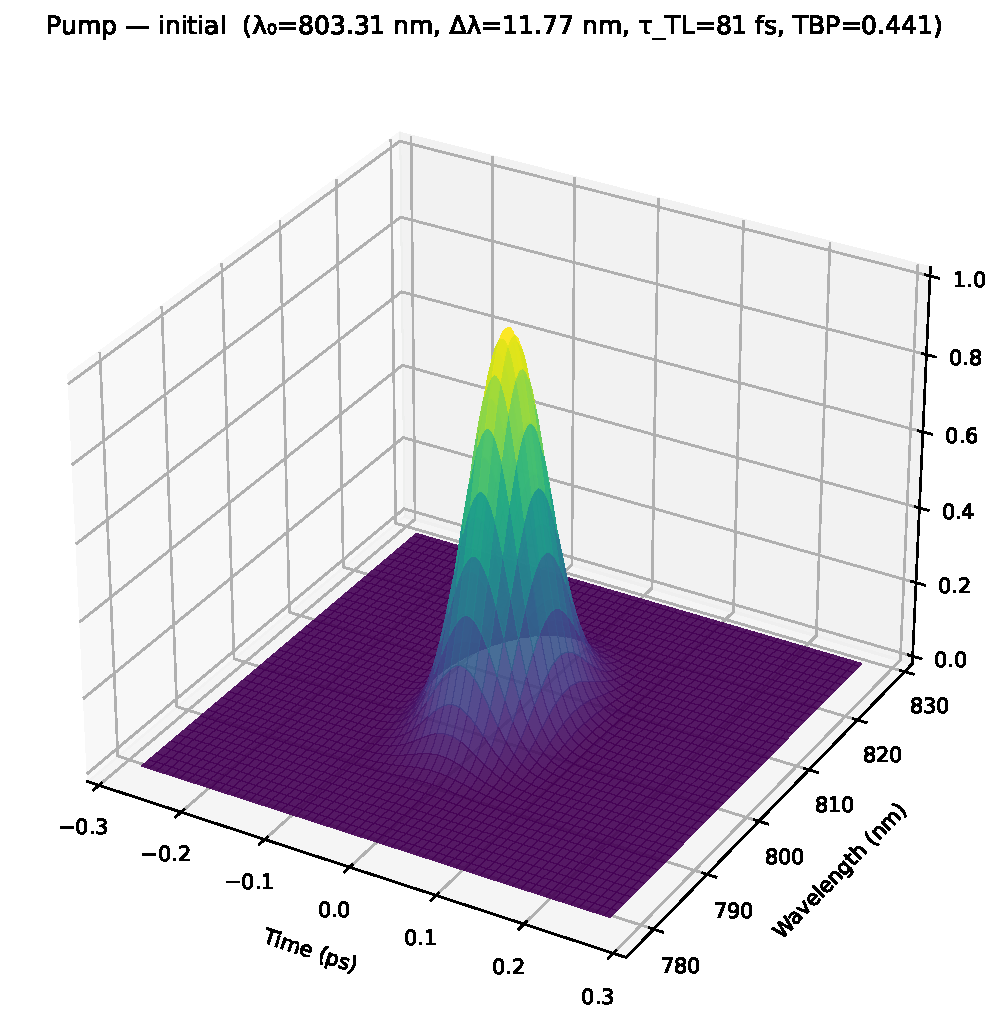
\includegraphics[width=0.90\textwidth, height=0.78\textheight, keepaspectratio]
    {../plots/resolution/pump_step0_initial.pdf}
\end{frame}

% ──────────────────────────────────────────────────────────────
% 5. TL STOKES — initial
% ──────────────────────────────────────────────────────────────
\begin{frame}{The Stokes pulse is transform-limited too, but twice as long at 1041 nm}
  \centering
  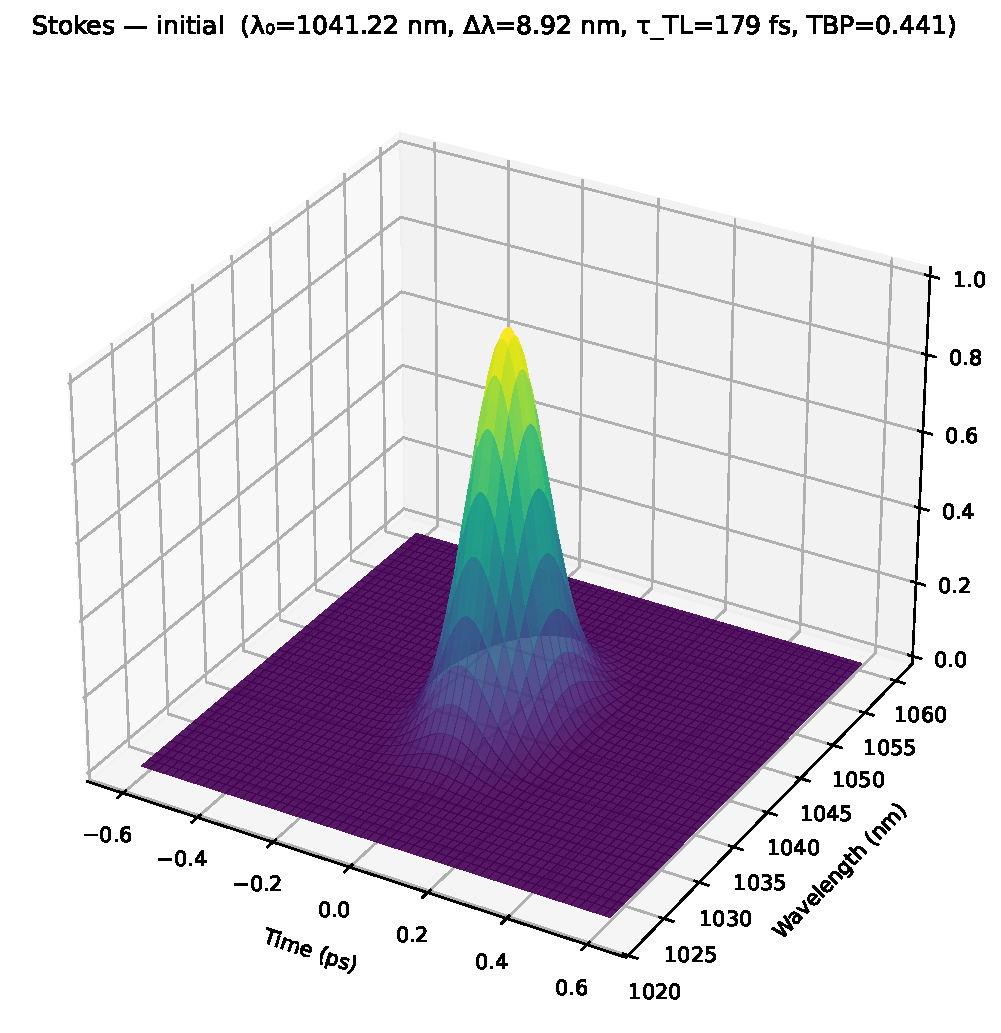
\includegraphics[width=0.90\textwidth, height=0.78\textheight, keepaspectratio]
    {../plots/resolution/stokes_step0_initial.pdf}
\end{frame}

% ──────────────────────────────────────────────────────────────
% 6. SIMULATION PIPELINE
% ──────────────────────────────────────────────────────────────
\begin{frame}{The simulation shifts each spectral slice by its group delay, then computes two convolutions}
  \centering
  \vspace{-0.2em}
  \[
    \tau_g(\lambda_i) = \frac{d\,\bigl[n_g(\lambda_i) - n_g(\lambda_0)\bigr]}{c},
    \quad n_g = n - \lambda\,\tfrac{dn}{d\lambda}
  \]
  \vspace{0.4em}
  \resizebox{0.97\textwidth}{!}{%
    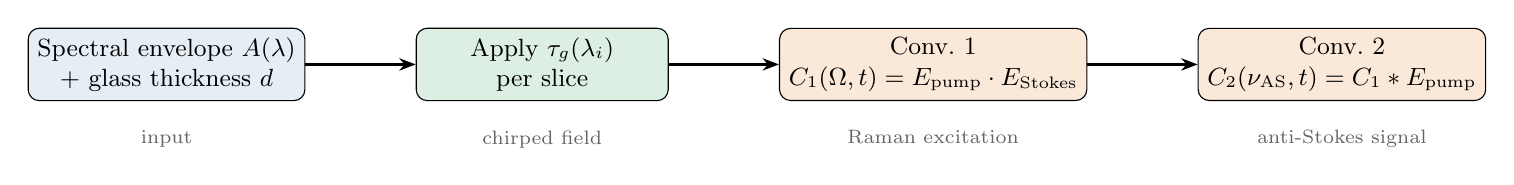
\begin{tikzpicture}[
      node distance=0.4cm and 1.2cm,
      box/.style ={draw, rounded corners=4pt, fill=mblue!10,
                   minimum width=3.2cm, minimum height=0.75cm,
                   font=\small, align=center},
      gbox/.style={draw, rounded corners=4pt, fill=mgreen!15,
                   minimum width=3.2cm, minimum height=0.75cm,
                   font=\small, align=center},
      obox/.style={draw, rounded corners=4pt, fill=morange!15,
                   minimum width=3.2cm, minimum height=0.75cm,
                   font=\small, align=center},
      arr/.style={-{Stealth[scale=0.9]}, thick},
      sub/.style={font=\scriptsize, mgray},
    ]
      \node[box]  (inp)  {Spectral envelope $A(\lambda)$\\+ glass thickness $d$};
      \node[gbox, right=1.4cm of inp]  (prop) {Apply $\tau_g(\lambda_i)$\\per slice};
      \node[obox, right=1.4cm of prop] (c1)   {Conv.\ 1\\$C_1(\Omega,t) = \Epump \cdot \Estokes$};
      \node[obox, right=1.4cm of c1]   (c2)   {Conv.\ 2\\$C_2(\nu_{\rm AS},t) = C_1 * \Epump$};
      \draw[arr] (inp)  -- (prop);
      \draw[arr] (prop) -- (c1);
      \draw[arr] (c1)   -- (c2);
      \node[sub, below=0.25cm of inp]   {input};
      \node[sub, below=0.25cm of prop]  {chirped field};
      \node[sub, below=0.25cm of c1]    {Raman excitation};
      \node[sub, below=0.25cm of c2]    {anti-Stokes signal};
    \end{tikzpicture}%
  }
  \vspace{0.5em}

  {\small All operations on \textbf{field amplitudes} ($E$), not intensities — CARS coherence scales as $\Epump \cdot \Estokes$.}
\end{frame}

% ──────────────────────────────────────────────────────────────
% 7. CHIRPED PUMP
% ──────────────────────────────────────────────────────────────
\begin{frame}{15 cm of S-TIH6 stretches the pump 52$\times$, mapping frequency onto time}
  \centering
  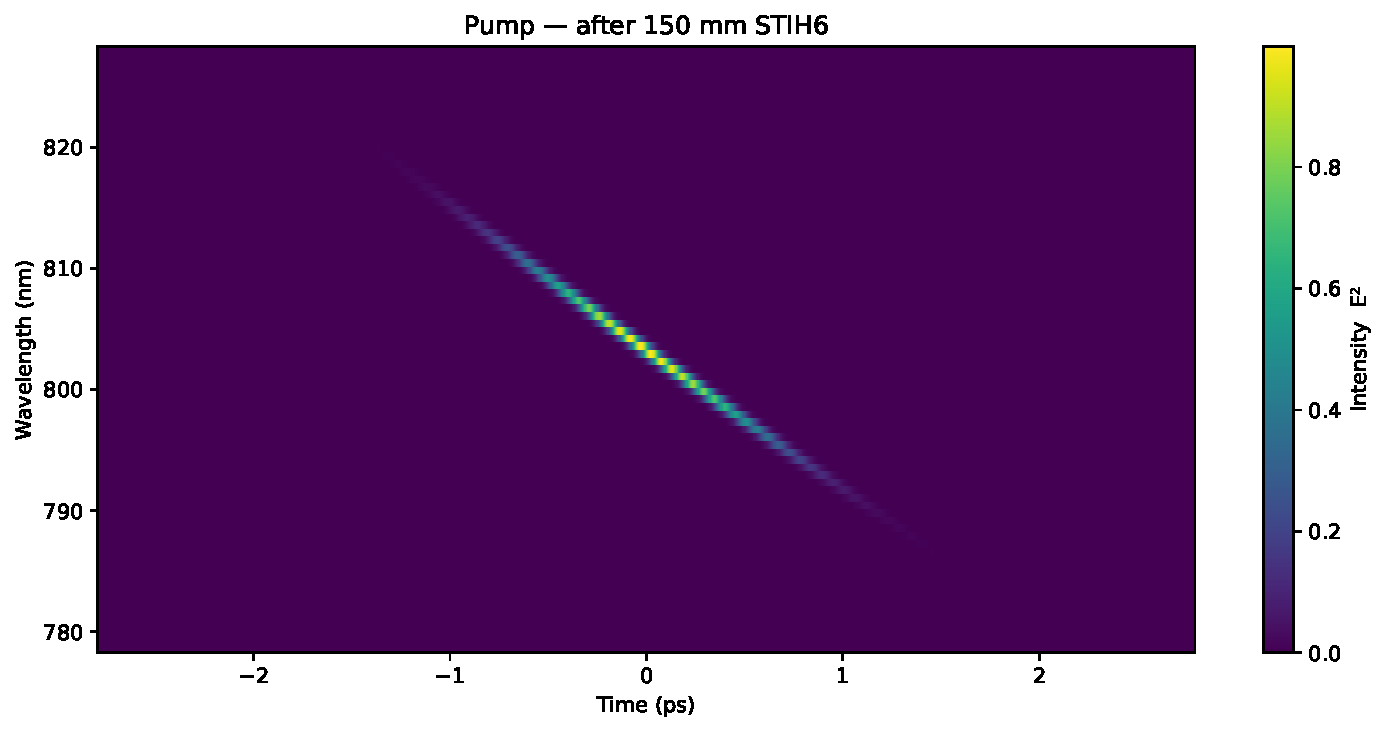
\includegraphics[width=0.90\textwidth, height=0.78\textheight, keepaspectratio]
    {../plots/resolution/pump_step1_propagated.pdf}
\end{frame}

% ──────────────────────────────────────────────────────────────
% 8. CHIRPED STOKES
% ──────────────────────────────────────────────────────────────
\begin{frame}{The same glass chirps the Stokes only 7$\times$: dispersion is weaker at 1041 nm}
  \centering
  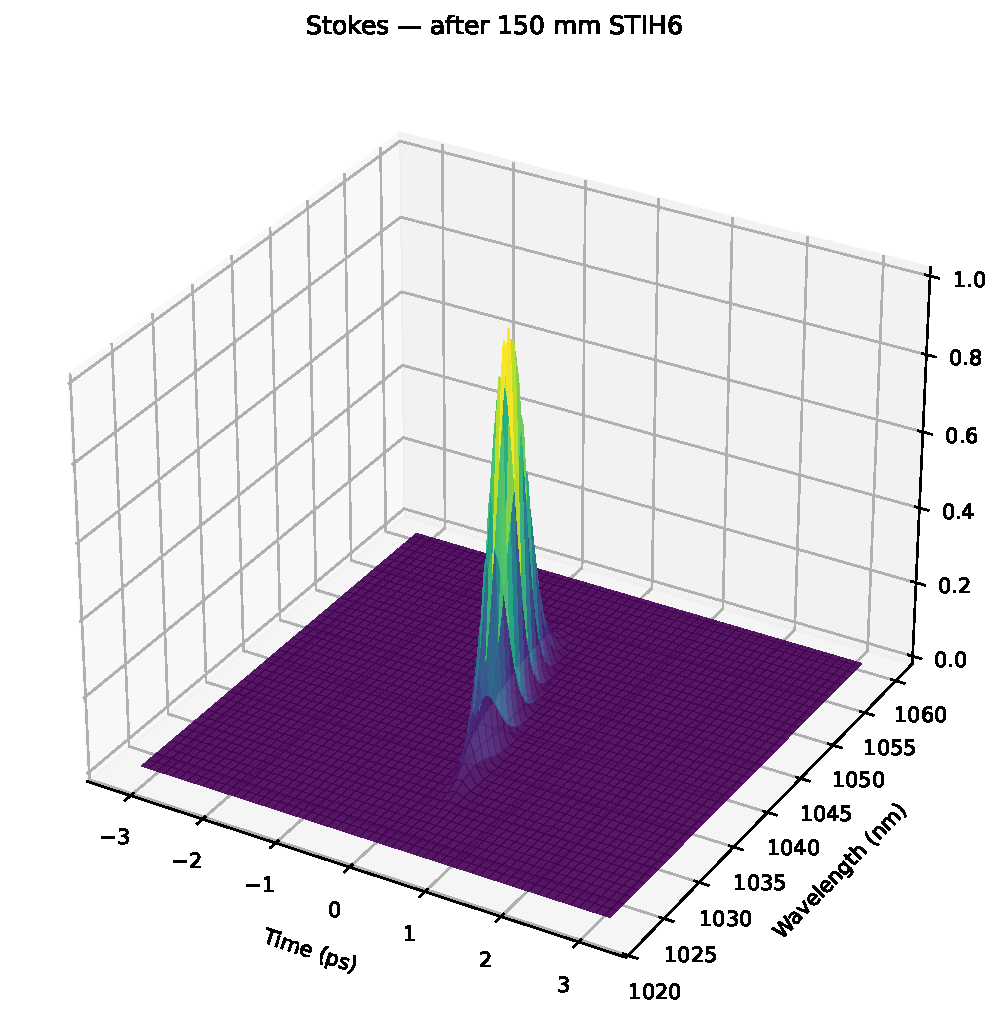
\includegraphics[width=0.90\textwidth, height=0.78\textheight, keepaspectratio]
    {../plots/resolution/stokes_step1_propagated.pdf}
\end{frame}

% ──────────────────────────────────────────────────────────────
% 9. PUMP MARGINAL
% ──────────────────────────────────────────────────────────────
\begin{frame}{Chirping costs 92\% of pump peak power — but total energy is conserved}
  \centering
  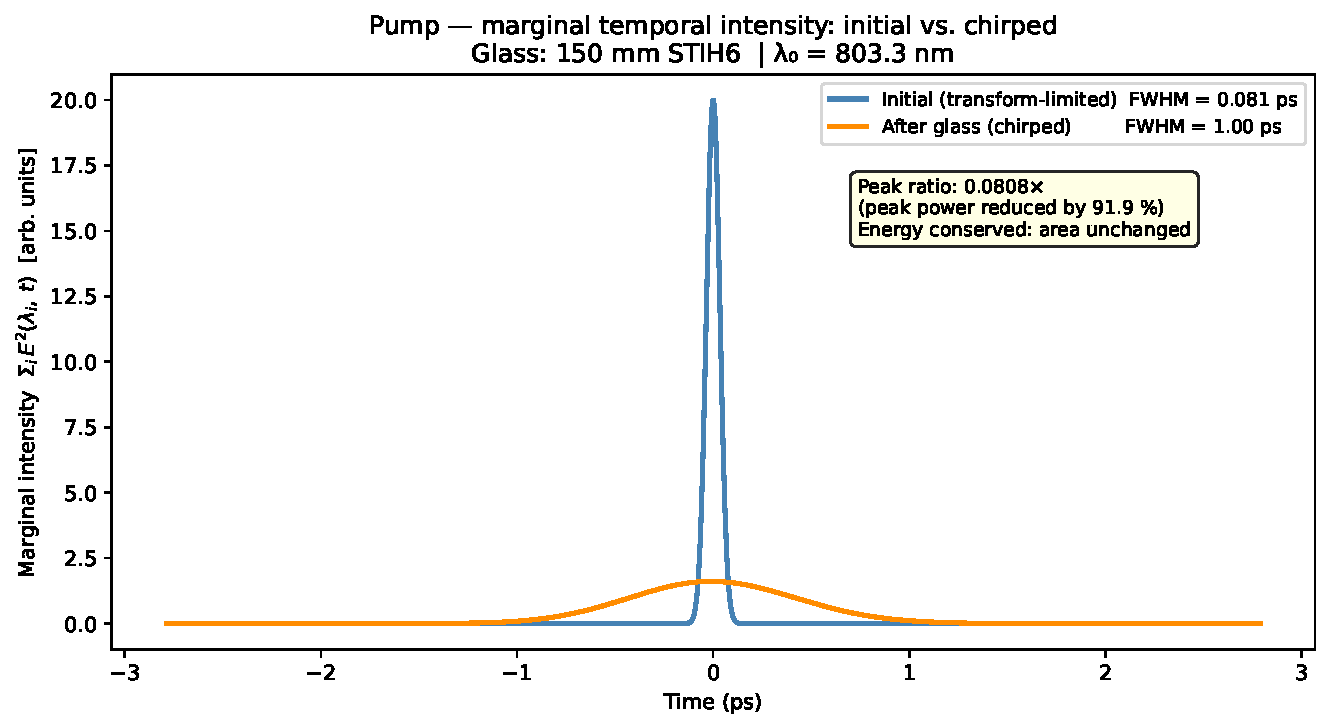
\includegraphics[width=0.90\textwidth, height=0.78\textheight, keepaspectratio]
    {../plots/resolution/pump_step1b_marginal.pdf}
\end{frame}

% ──────────────────────────────────────────────────────────────
% 10. STOKES MARGINAL
% ──────────────────────────────────────────────────────────────
\begin{frame}{Stokes loses only 49\% of peak power: it sweeps frequency more slowly}
  \centering
  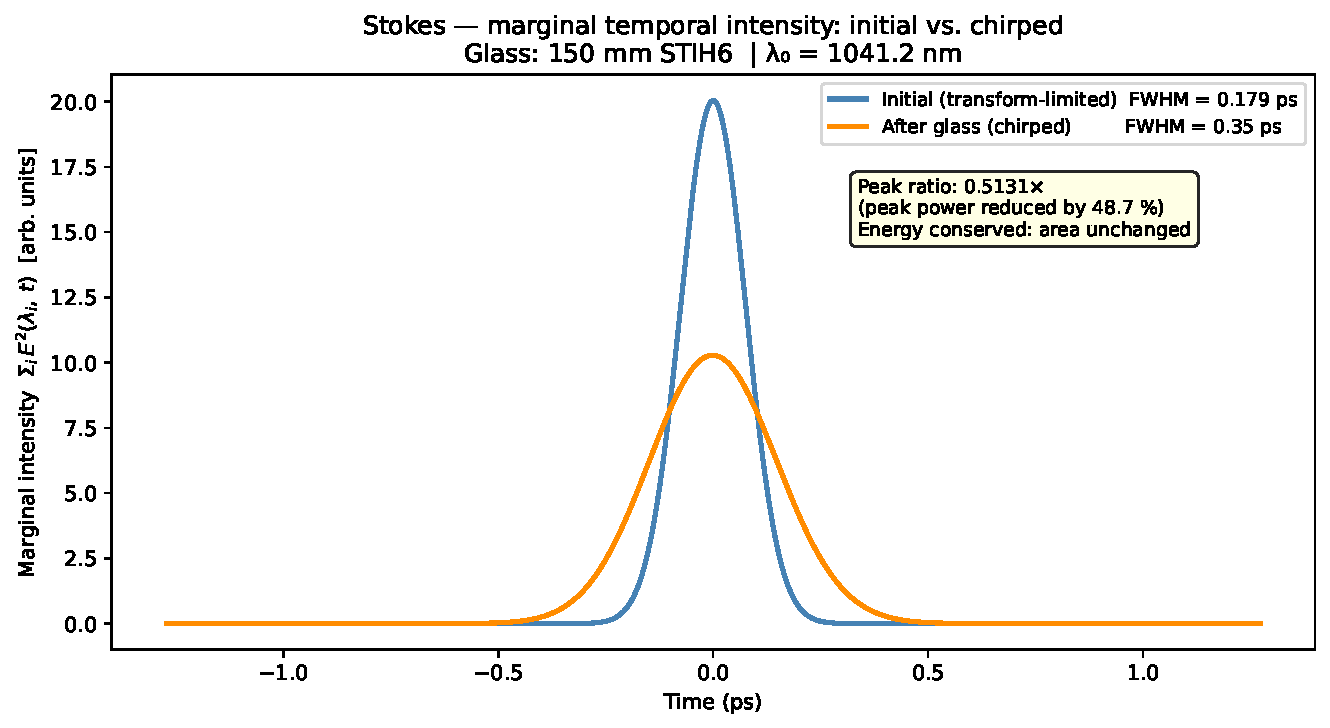
\includegraphics[width=0.90\textwidth, height=0.78\textheight, keepaspectratio]
    {../plots/resolution/stokes_step1b_marginal.pdf}
\end{frame}

% ──────────────────────────────────────────────────────────────
% 11. C1 ZERO DELAY
% ──────────────────────────────────────────────────────────────
\begin{frame}{At each instant a single Raman mode is driven: the horizontal ridge is spectral focusing}
  \centering
  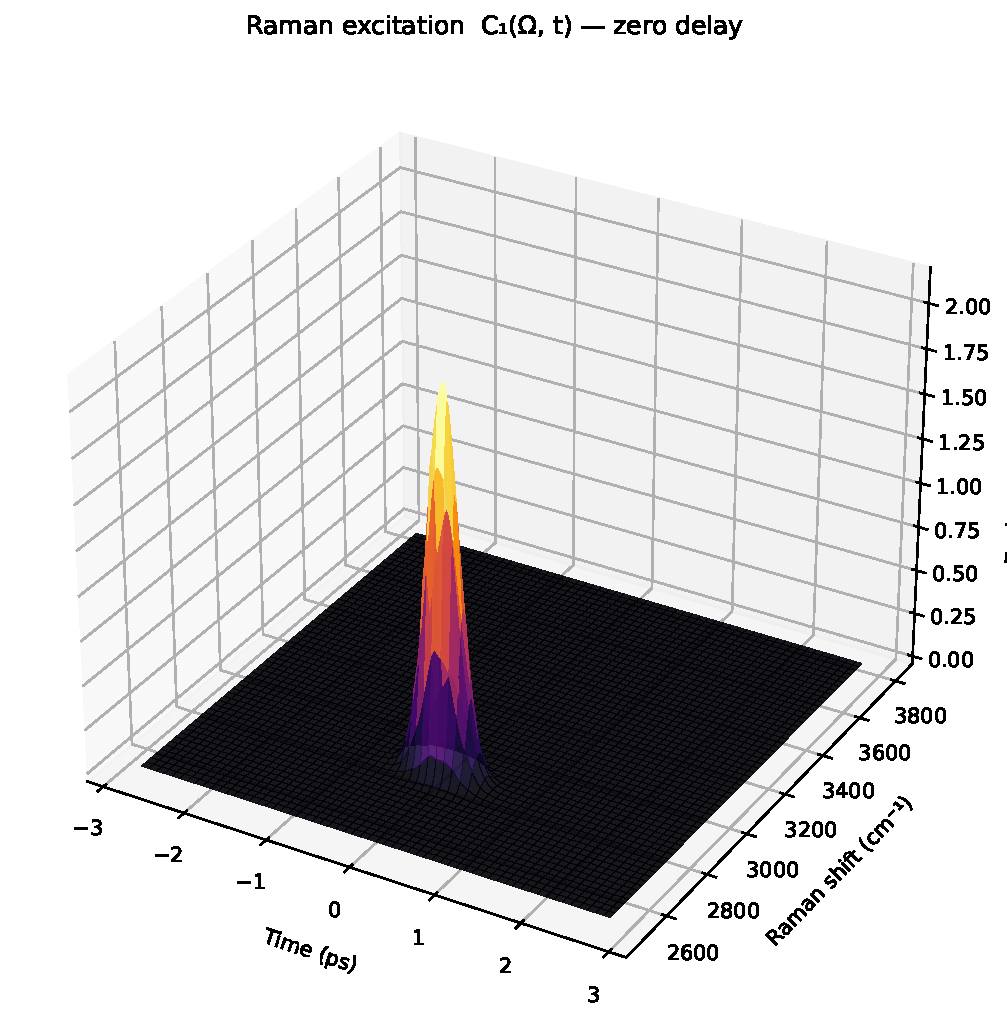
\includegraphics[width=0.90\textwidth, height=0.78\textheight, keepaspectratio]
    {../plots/resolution/conv1_zero_delay.pdf}
\end{frame}

% ──────────────────────────────────────────────────────────────
% 12. C1 OPTIMAL DELAY
% ──────────────────────────────────────────────────────────────
\begin{frame}{Optimal delay is zero: matched chirp rates naturally align the two beams}
  \centering
  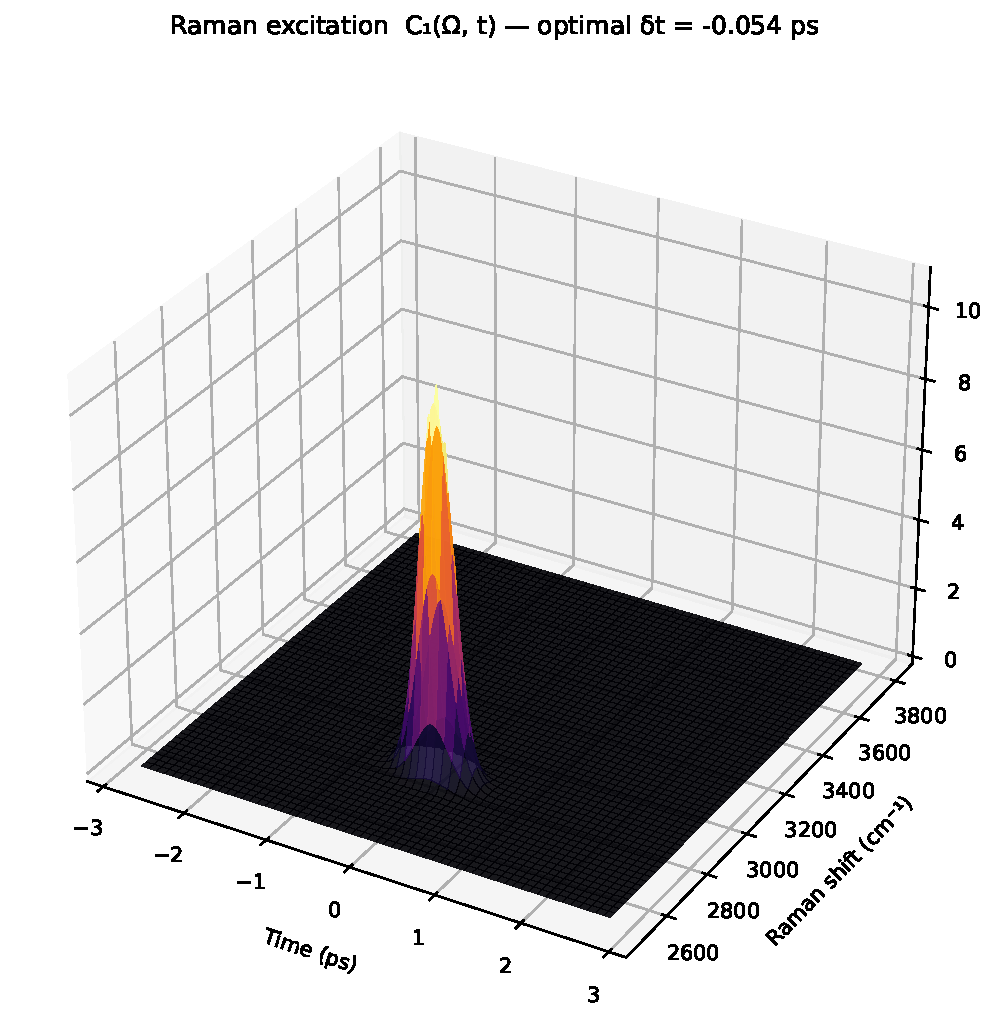
\includegraphics[width=0.90\textwidth, height=0.78\textheight, keepaspectratio]
    {../plots/resolution/conv1_optimal_delay.pdf}
\end{frame}

% ──────────────────────────────────────────────────────────────
% 13. C1 COMPARISON
% ──────────────────────────────────────────────────────────────
\begin{frame}{Matched chirp delivers 27.1\,cm\textsuperscript{$-1$} Raman resolution — and timing barely matters}
  \centering
  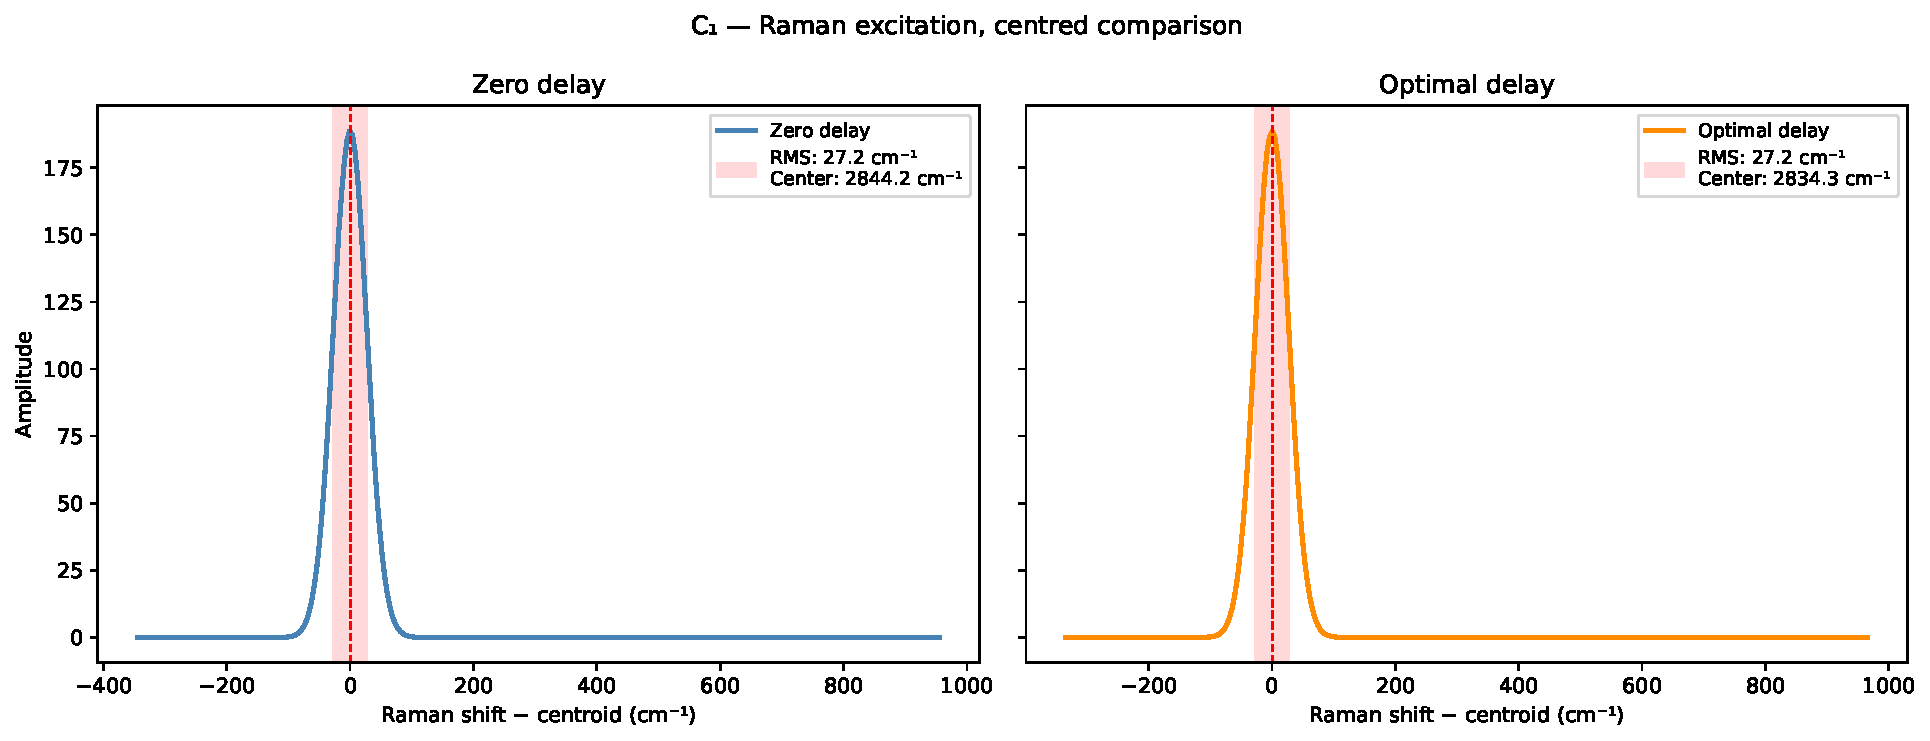
\includegraphics[width=0.90\textwidth, height=0.78\textheight, keepaspectratio]
    {../plots/resolution/comparison_c1.pdf}
\end{frame}

% ──────────────────────────────────────────────────────────────
% 14. C2 ZERO + OPTIMAL SIDE BY SIDE
% ──────────────────────────────────────────────────────────────
\begin{frame}{The probe pump converts Raman coherence into anti-Stokes light at 654 nm}
  \begin{columns}[c]
    \column{0.47\textwidth}
      \centering
      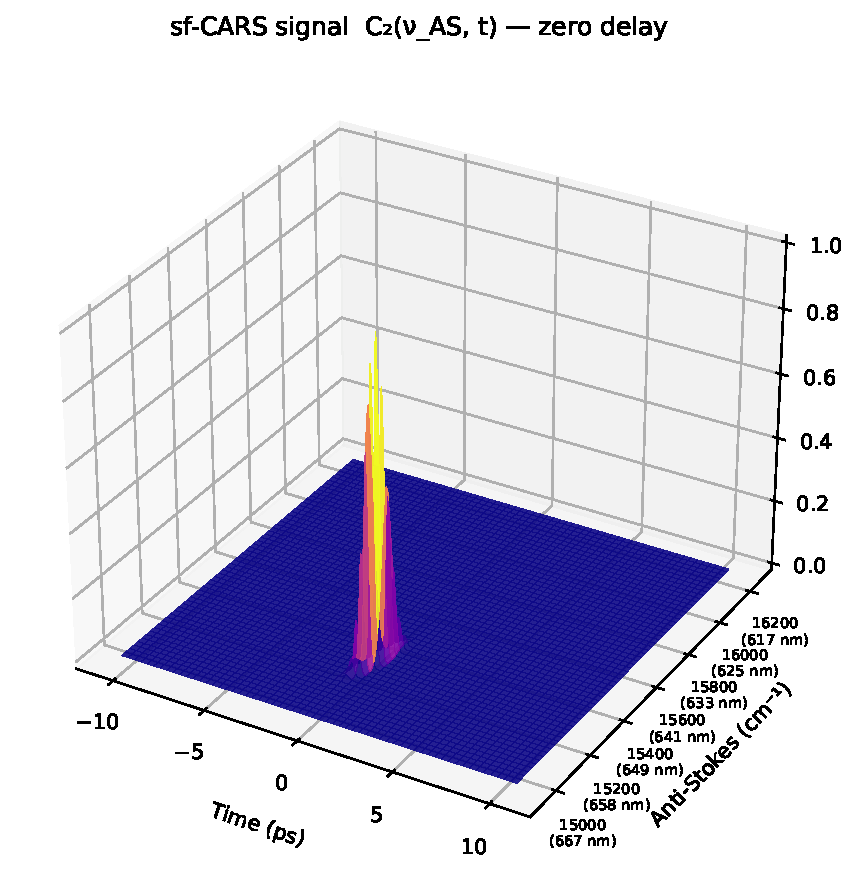
\includegraphics[width=\linewidth, height=0.65\textheight, keepaspectratio]
        {../plots/resolution/conv2_zero_delay.pdf}\\[0.3em]
      {\small Zero delay}
    \column{0.47\textwidth}
      \centering
      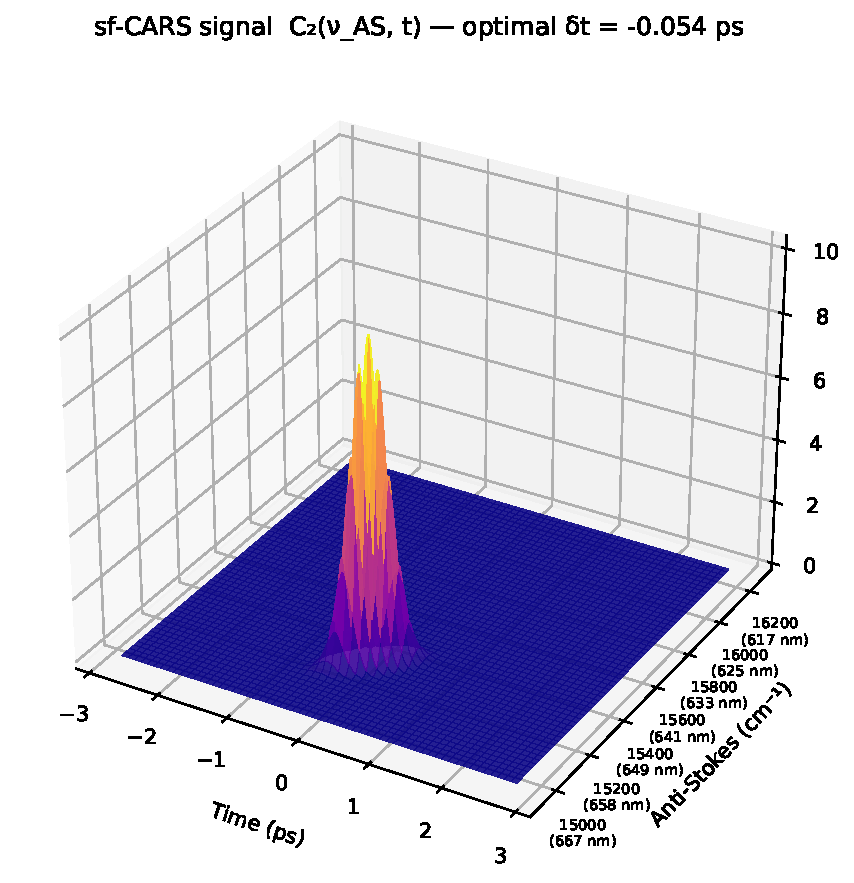
\includegraphics[width=\linewidth, height=0.65\textheight, keepaspectratio]
        {../plots/resolution/conv2_optimal_delay.pdf}\\[0.3em]
      {\small Optimal delay ($\delta t^\star \approx 0$)}
  \end{columns}
\end{frame}

% ──────────────────────────────────────────────────────────────
% 15. C2 PROJECTIONS SIDE BY SIDE
% ──────────────────────────────────────────────────────────────
\begin{frame}{Both delays yield the same 41.5\,cm\textsuperscript{$-1$} anti-Stokes linewidth}
  \begin{columns}[c]
    \column{0.47\textwidth}
      \centering
      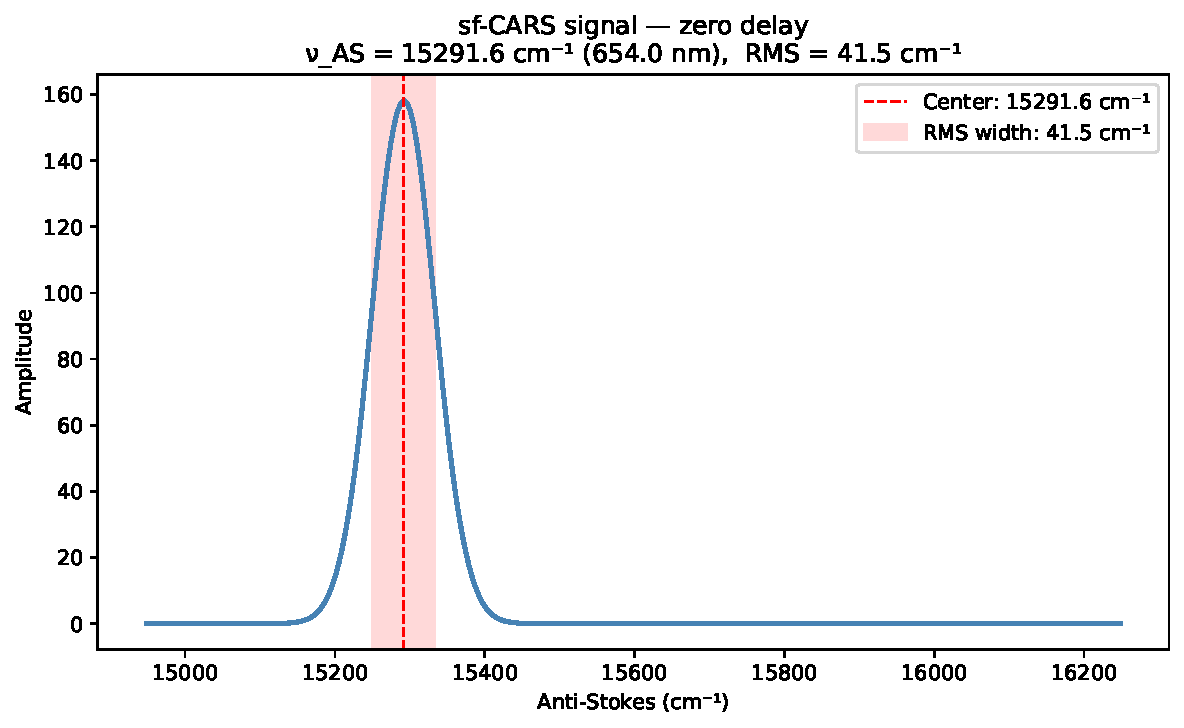
\includegraphics[width=\linewidth, height=0.65\textheight, keepaspectratio]
        {../plots/resolution/conv2_zero_delay_projection.pdf}\\[0.3em]
      {\small Zero delay}
    \column{0.47\textwidth}
      \centering
      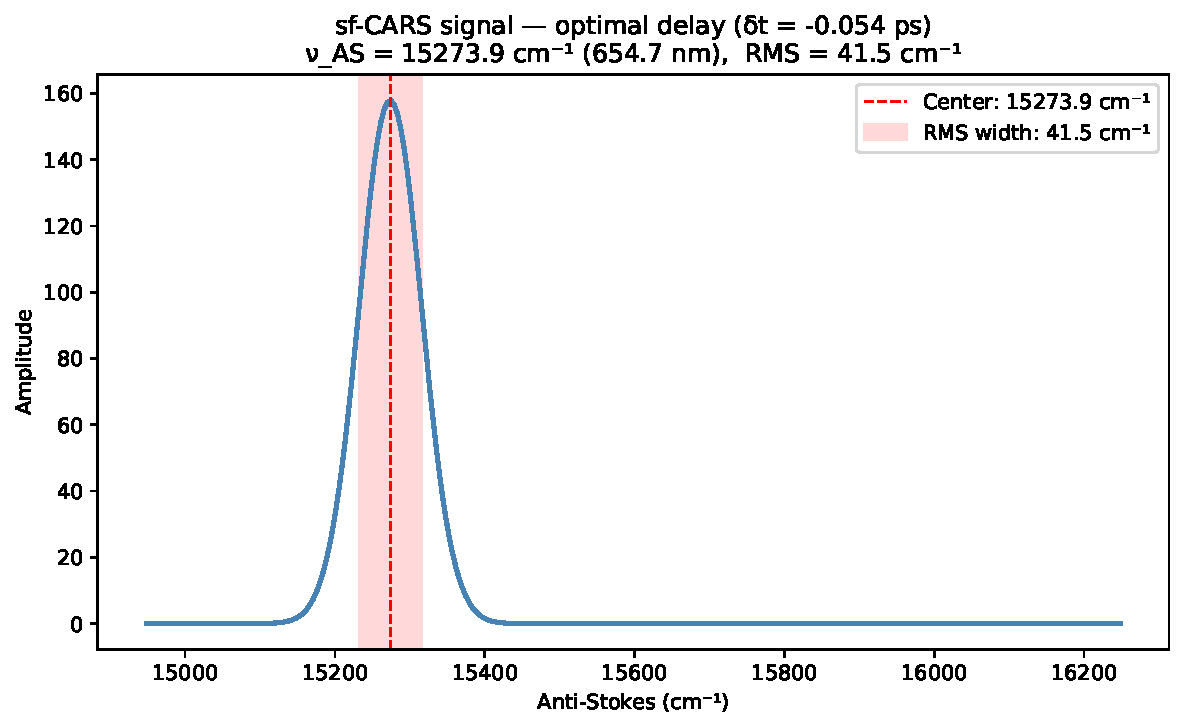
\includegraphics[width=\linewidth, height=0.65\textheight, keepaspectratio]
        {../plots/resolution/conv2_optimal_delay_projection.pdf}\\[0.3em]
      {\small Optimal delay — \textbf{RMS\,=\,41.5\,cm$^{-1}$}}
  \end{columns}
\end{frame}

% ──────────────────────────────────────────────────────────────
% 16. C2 COMPARISON (SCENARIO A)
% ──────────────────────────────────────────────────────────────
\begin{frame}{The degenerate probe broadens the anti-Stokes spectrum 53\% beyond $C_1$}
  \centering
  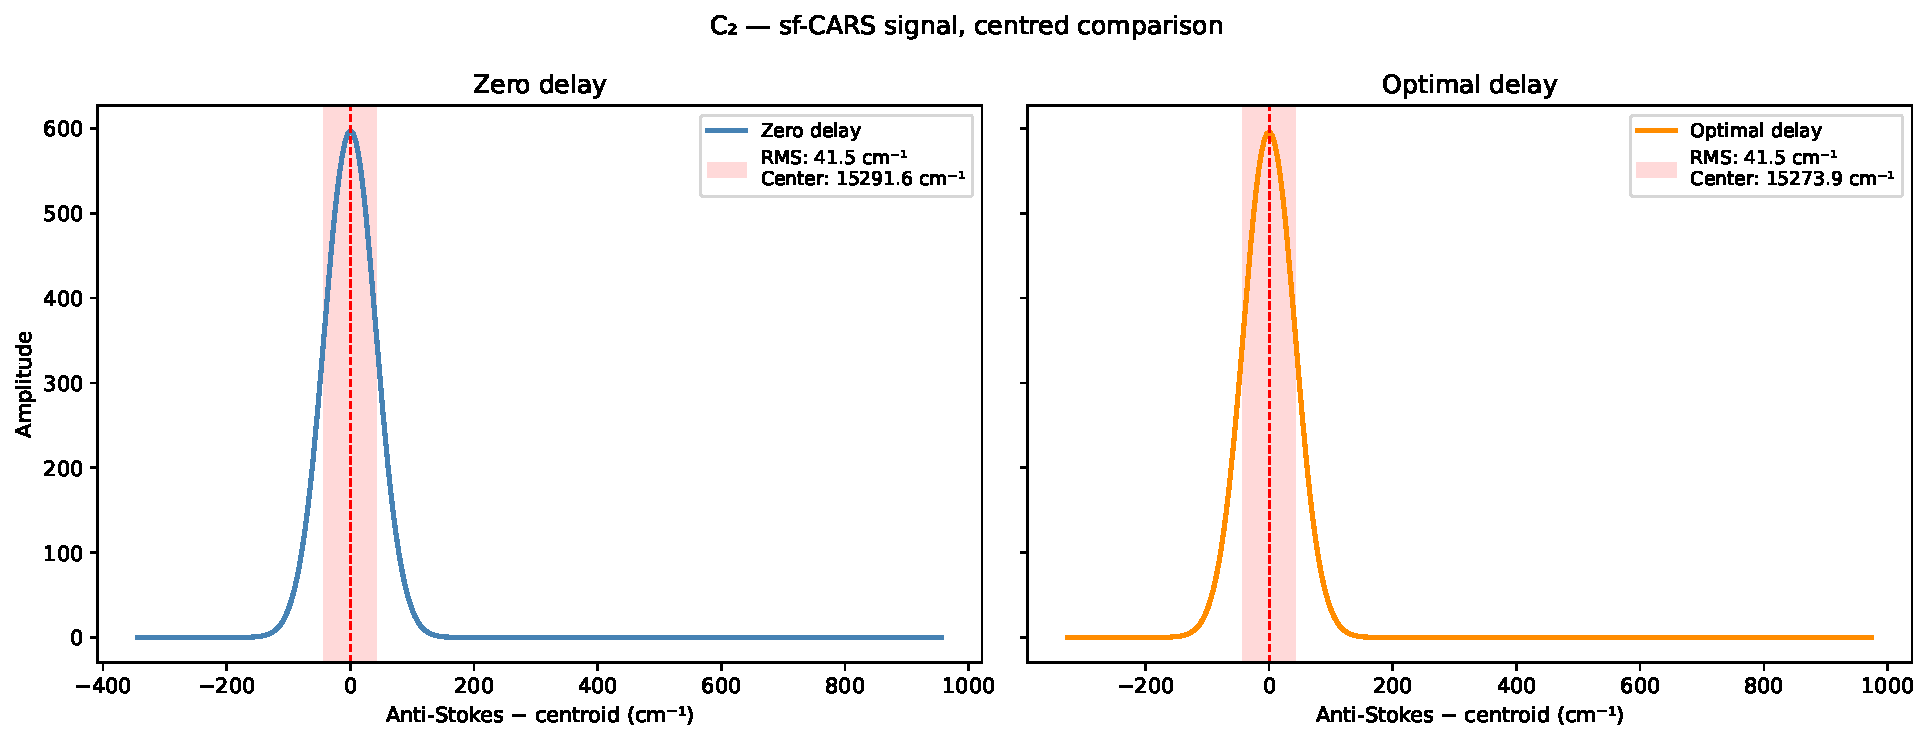
\includegraphics[width=0.90\textwidth, height=0.78\textheight, keepaspectratio]
    {../plots/resolution/comparison_c2.pdf}
\end{frame}

% ──────────────────────────────────────────────────────────────
% 17. C1 COMPARISON A vs B
% ──────────────────────────────────────────────────────────────
\begin{frame}{Halving pump glass from 15 to 5 cm doubles the Raman excitation linewidth}
  \begin{columns}[c]
    \column{0.47\textwidth}
      \centering
      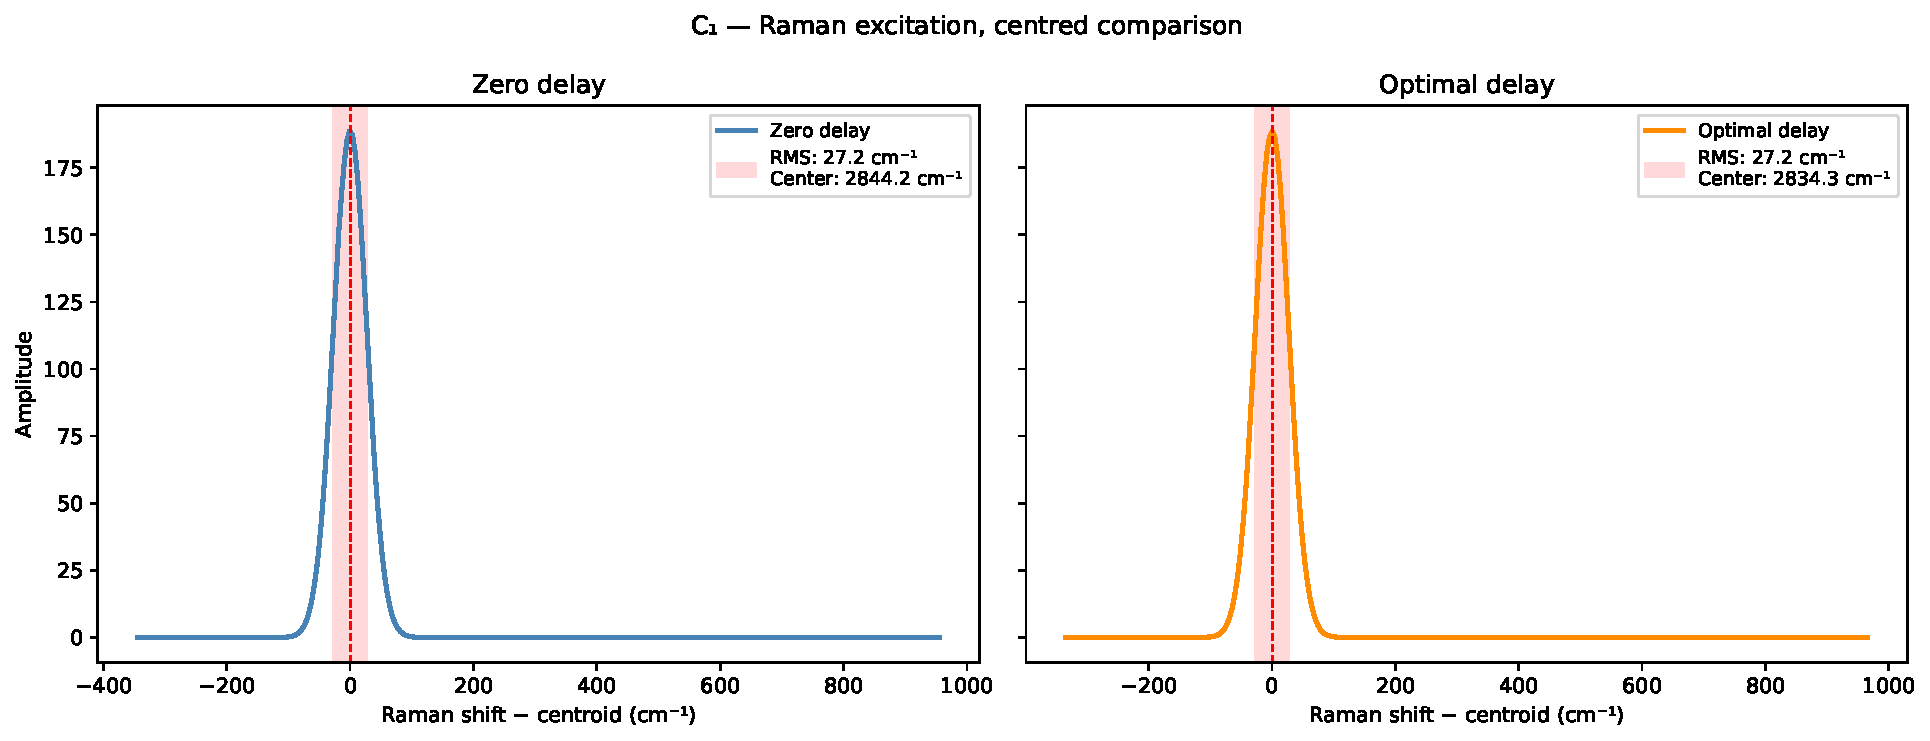
\includegraphics[width=\linewidth, height=0.65\textheight, keepaspectratio]
        {../plots/resolution/comparison_c1.pdf}\\[0.3em]
      {\small \textbf{Scenario A} — pump 15 cm\\[0.2em] \textbf{RMS\,=\,27.1\,cm$^{-1}$}}
    \column{0.47\textwidth}
      \centering
      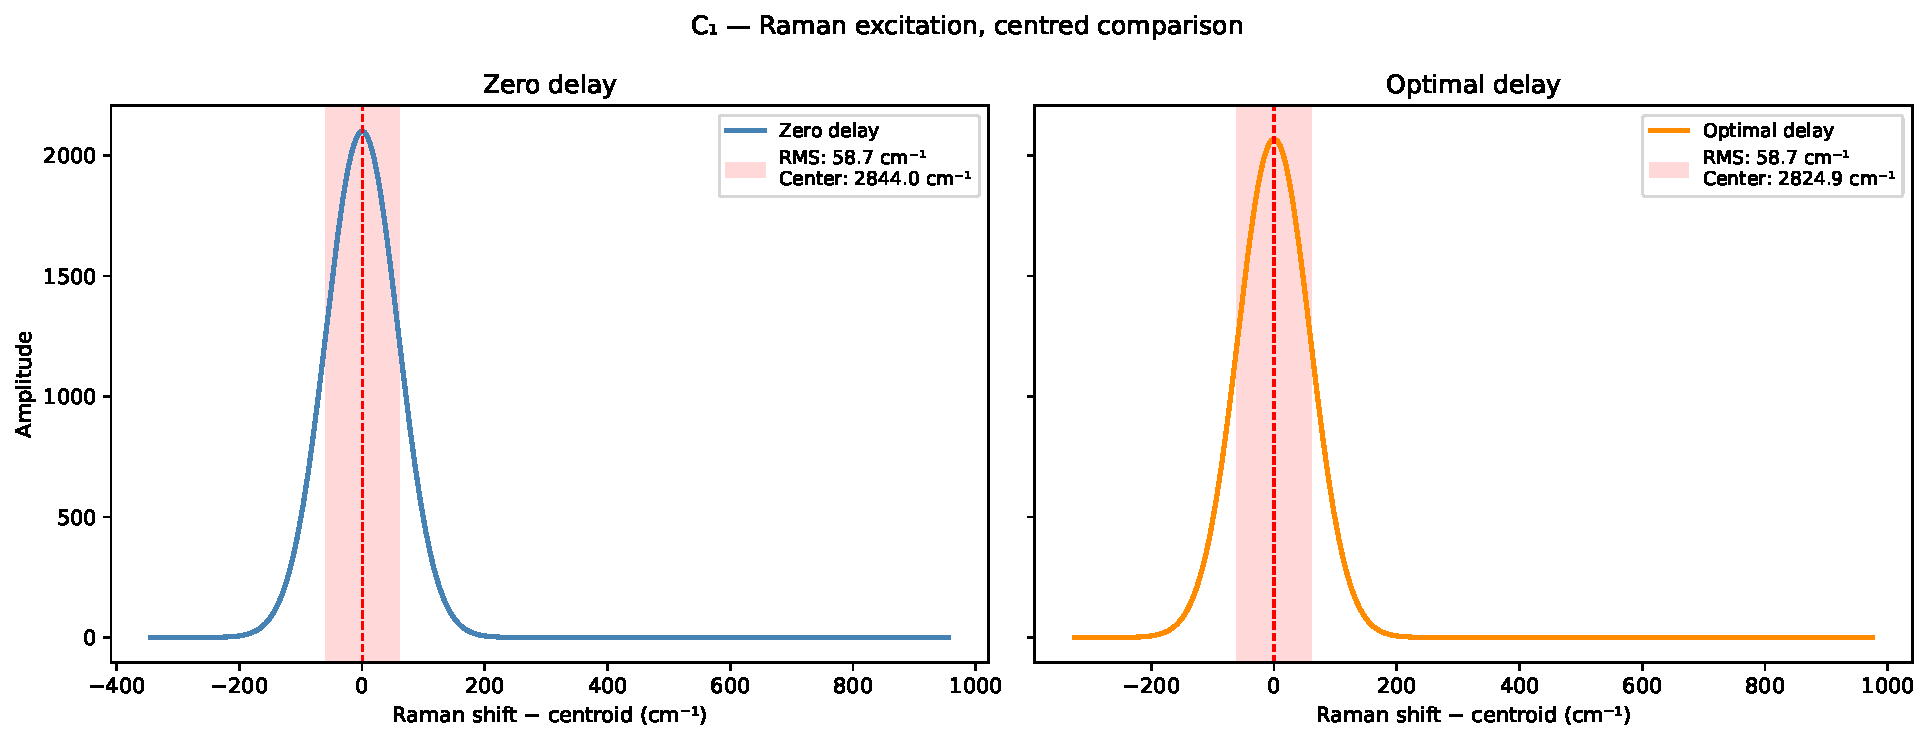
\includegraphics[width=\linewidth, height=0.65\textheight, keepaspectratio]
        {../plots/resolution_pump5cm/comparison_c1.pdf}\\[0.3em]
      {\small \textbf{Scenario B} — pump 5 cm\\[0.2em] \textbf{RMS\,=\,58.7\,cm$^{-1}$}}
  \end{columns}
\end{frame}

% ──────────────────────────────────────────────────────────────
% 18. C2 COMPARISON A vs B
% ──────────────────────────────────────────────────────────────
\begin{frame}{Mismatched chirp degrades anti-Stokes resolution 2.6$\times$}
  \begin{columns}[c]
    \column{0.47\textwidth}
      \centering
      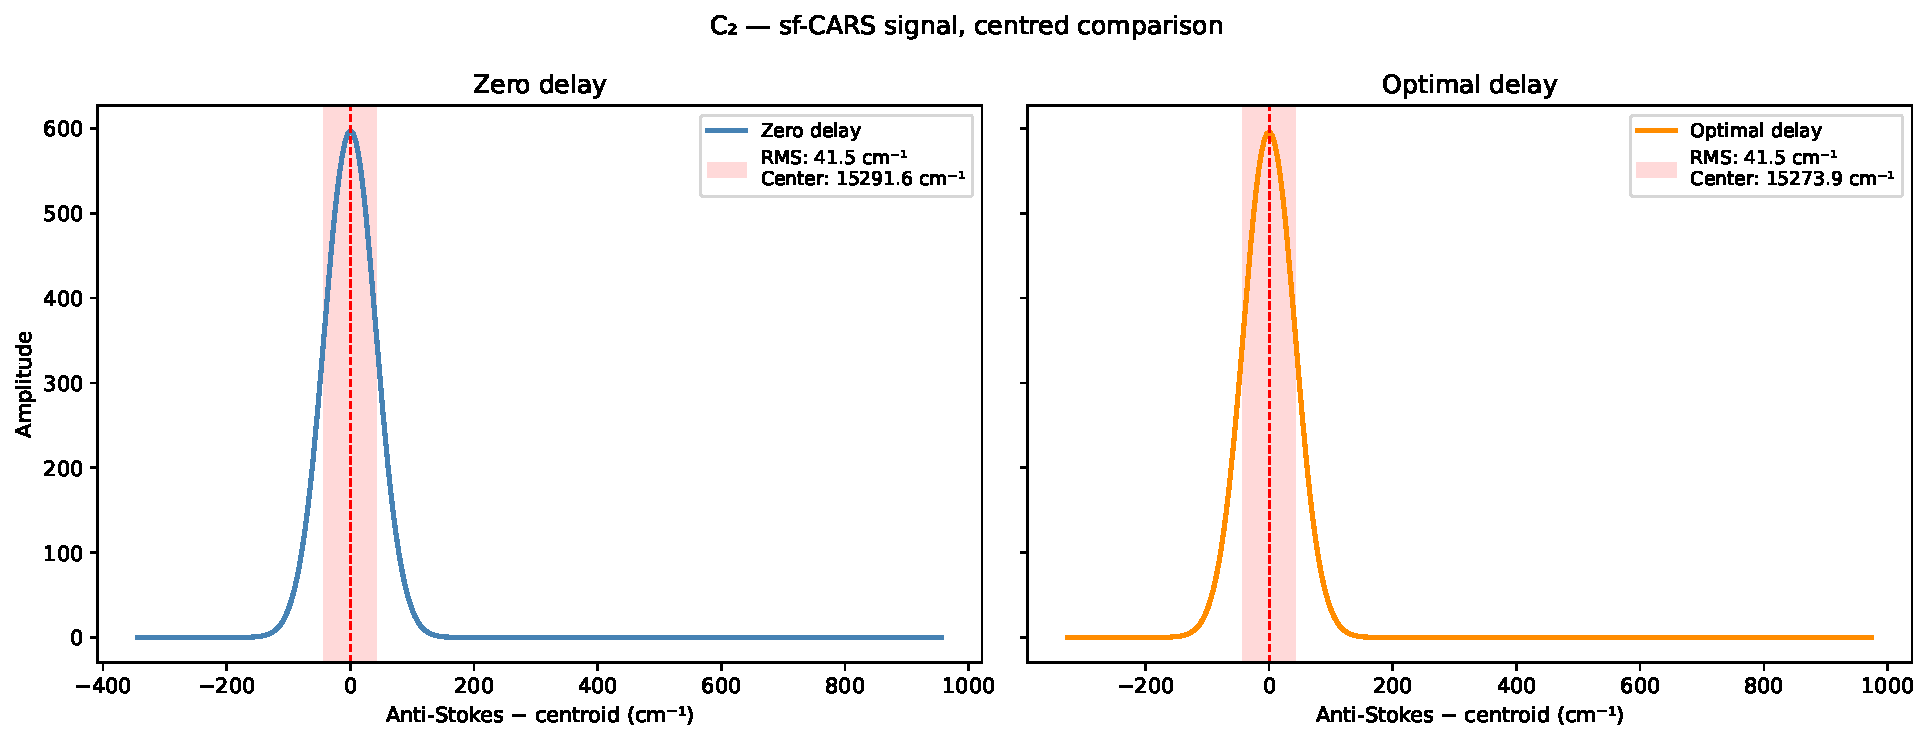
\includegraphics[width=\linewidth, height=0.65\textheight, keepaspectratio]
        {../plots/resolution/comparison_c2.pdf}\\[0.3em]
      {\small \textbf{Scenario A} — pump 15 cm\\[0.2em] \textbf{RMS\,=\,41.5\,cm$^{-1}$}}
    \column{0.47\textwidth}
      \centering
      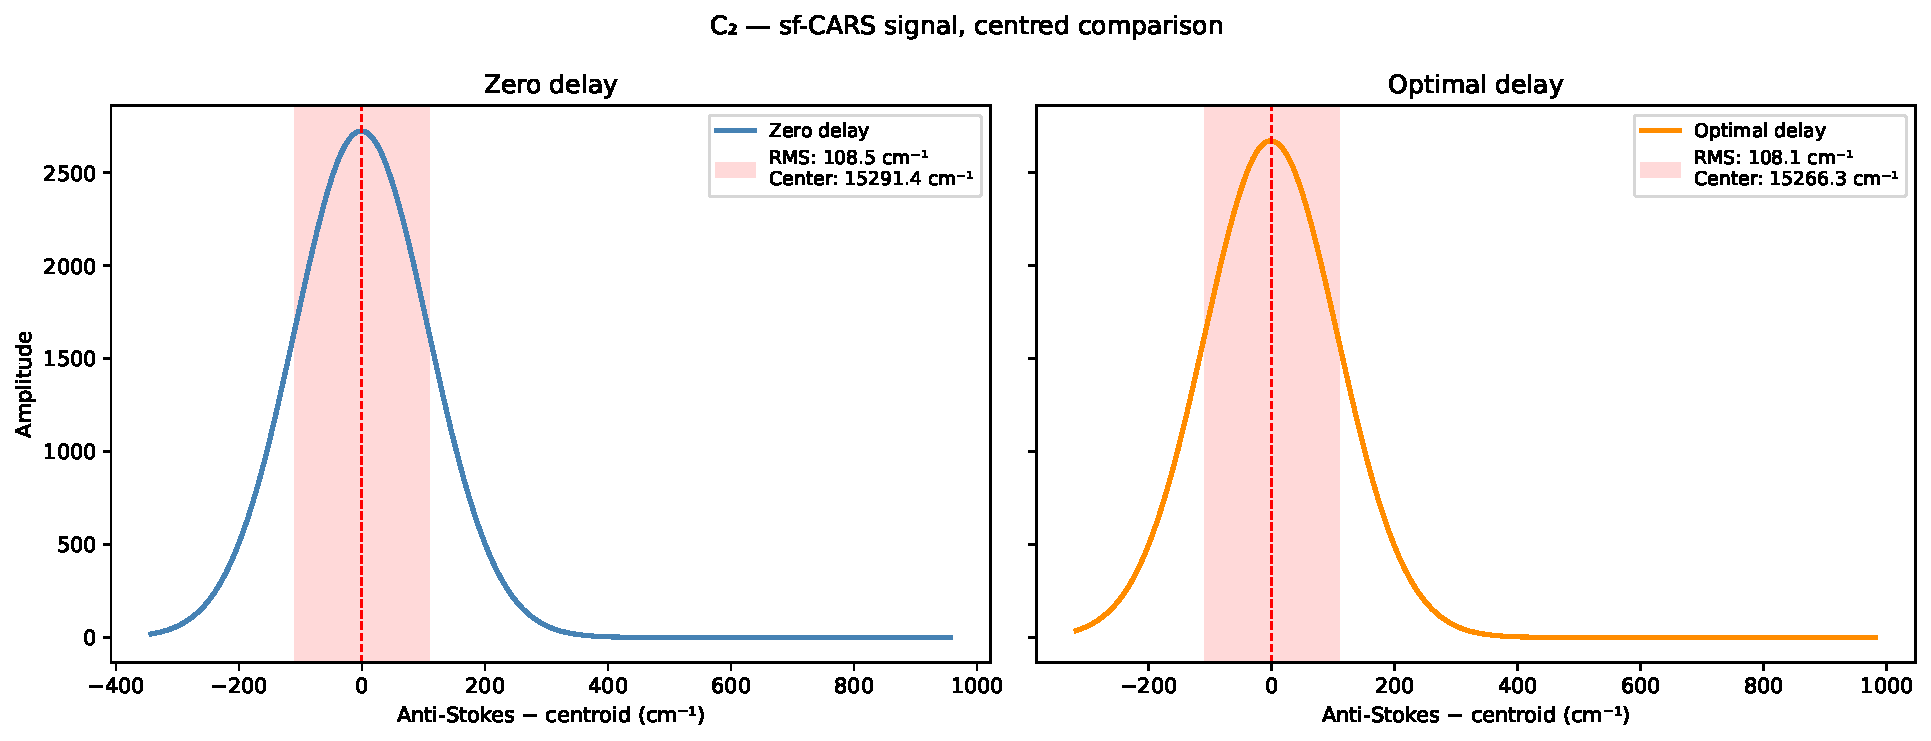
\includegraphics[width=\linewidth, height=0.65\textheight, keepaspectratio]
        {../plots/resolution_pump5cm/comparison_c2.pdf}\\[0.3em]
      {\small \textbf{Scenario B} — pump 5 cm\\[0.2em] \textbf{RMS\,=\,108.5\,cm$^{-1}$}}
  \end{columns}
\end{frame}

% ──────────────────────────────────────────────────────────────
% 19. SUMMARY TABLE
% ──────────────────────────────────────────────────────────────
\begin{frame}{More pump glass: $2.6\times$ better resolution, $3\times$ lower peak power — the same knob controls both}
  \begin{columns}[T]
    \column{0.60\textwidth}
      \vspace{0.2em}
      \renewcommand{\arraystretch}{1.25}
      \begin{table}
        \centering\small
        \begin{tabular}{lcc}
          \toprule
          & \textbf{Scenario A} & \textbf{Scenario B} \\
          & \footnotesize pump 15 cm & \footnotesize pump 5 cm \\
          \midrule
          Pump GD spread     & \SI{4.21}{ps}           & \SI{1.40}{ps} \\
          Pump elongation    & $\approx 52\times$      & $\approx 17\times$ \\
          Pump peak ratio    & 0.080 \;($-92\%$)       & 0.22\phantom{0} \;($-78\%$) \\
          \midrule
          $C_1$ RMS ($\wn$)  & \textbf{27.1}           & \textbf{58.7} \\
          $C_2$ RMS ($\wn$)  & \textbf{41.5}           & \textbf{108.5} \\
          Optimal $\delta t$ & $\approx 0$             & $\neq 0$ \\
          \bottomrule
        \end{tabular}
      \end{table}

    \column{0.37\textwidth}
      \vspace{0.8em}
      \alert{Chirp matching ($2\times$ glass ratio) gives $2.2\times$ better $C_1$ resolution.}

      \vspace{0.6em}
      \alert{Anti-Stokes ($C_2$) improves $2.6\times$ — only Stokes glass is fixed.}

      \vspace{0.6em}
      \alert{More glass $\Rightarrow$ narrower linewidth \emph{and} lower signal.}
  \end{columns}
\end{frame}

% ──────────────────────────────────────────────────────────────
% 20. CONCLUSIONS
% ──────────────────────────────────────────────────────────────
\begin{frame}{Spectral focusing turns femtosecond bandwidth into narrowband Raman sensitivity — chirp matching is the key}
  \begin{enumerate}
    \setlength{\itemsep}{0.60em}
    \item \textbf{S-TIH6 imprints a linear frequency-to-time map.}
          Pump: $80\,\text{fs} \to 4.2\,\text{ps}$ ($52\times$); Stokes: $179\,\text{fs} \to 1.3\,\text{ps}$ ($7\times$).
    \item \textbf{Peak power drops but energy is conserved.}
          Pump peak ratio $= 0.080 = 1/\neff$; \;$\int I\,dt$ ratio $= 1.000$.
    \item \textbf{Matched chirp rates achieve 27\,cm$^{-1}$ Raman resolution}
          from an 11.77 nm input bandwidth — the time-frequency mapping acts as a narrowband filter.
    \item \textbf{Mismatch is costly.}
          Pump 5 vs.\ 15 cm: $C_1$ degrades $2.2\times$, $C_2$ degrades $2.6\times$.
    \item \textbf{The degenerate probe adds 53\% spectral width.}
          $C_2$ RMS $=41.5\wn > C_1$ RMS $=27.1\wn$; a narrowband probe would sharpen the final spectrum.
  \end{enumerate}
\end{frame}

% ──────────────────────────────────────────────────────────────
% 21. CLOSING
% ──────────────────────────────────────────────────────────────
\begin{frame}[standout]
  \Huge Thank you

  \vspace{0.7em}
  \large Questions?

  \vspace{1.2em}
  \normalsize
  Code: branch \texttt{3d-propagation} \;—\; \texttt{resolution.py}\\[0.4em]
  All plots and simulation scripts available in the repository.
\end{frame}

% ============================================================
\end{document}
